%!TEX root = ../crimson_throne_book_main.tex
% 2015-09-26
The companions return to Vencarlo's burned down academy and build a pyre for Alika. Sjo prays to Pharasma to show mercy on the poor, misguided girl's soul and Quint pours his sorrow in a sad song. Balian just watches in silence as his sister's remains are consumed by the flames, hoping that she will find some kind of peace in the afterlife. Afterwards the party heads to the Endrin Academy, where Amin Jalento, Korwick and Heldrin are still safe. The sadness of Alika's demise is somewhat compensated by the joy of Mouse, reconnecting with his two best friends. Realising that they accomplished nearly the impossible by saving the three boys from the clutches of death definitely brings some comfort. Weary of today's trials, our heroes quickly slink away in sleep's embrace.\\

\section{22 Erastus 4708}

The next morning immediately proves how resilient young boys can be. Although they went through a traumatizing experience, Korwick, Mouse and Heldrin do not appear dazed. Sjo feels proud when he sees that his wards put food first in their priorities, plundering the provision cabinet for salami. Having faced the revenge of a deranged necromancer did not break little Mouse, as he recounts to his friends how the heroes saved him from the bad man with much gusto. Who knows, these boys might have the making of heroes in their hearts as well.\\

Following up on Amin Jalento's hint that Salvator Scream, the painter, visited his master Vencarlo Orisini on several occasions,\hyperref[fig:Where-is-Salvator-Scream-562539967]{ the companions head over to the artist's house } . The decripit building on the Narrows of Saint Alika appears in an even sadder state than the last time the party came here. As Balian moves in to pry open the lock on the front door, he notices that someone beat him to the punch. It looks like Salvator Scream already had 'visitors' a couple of days ago. The door swings open to reveal a front room with multiple muddy tracks covering the floorboards. The footprints lead to the bedroom with a single bed. The blankets and pillow atop are in disarray and there is no sign of the painter. \\

\begin{figure}[h]
	\centering
	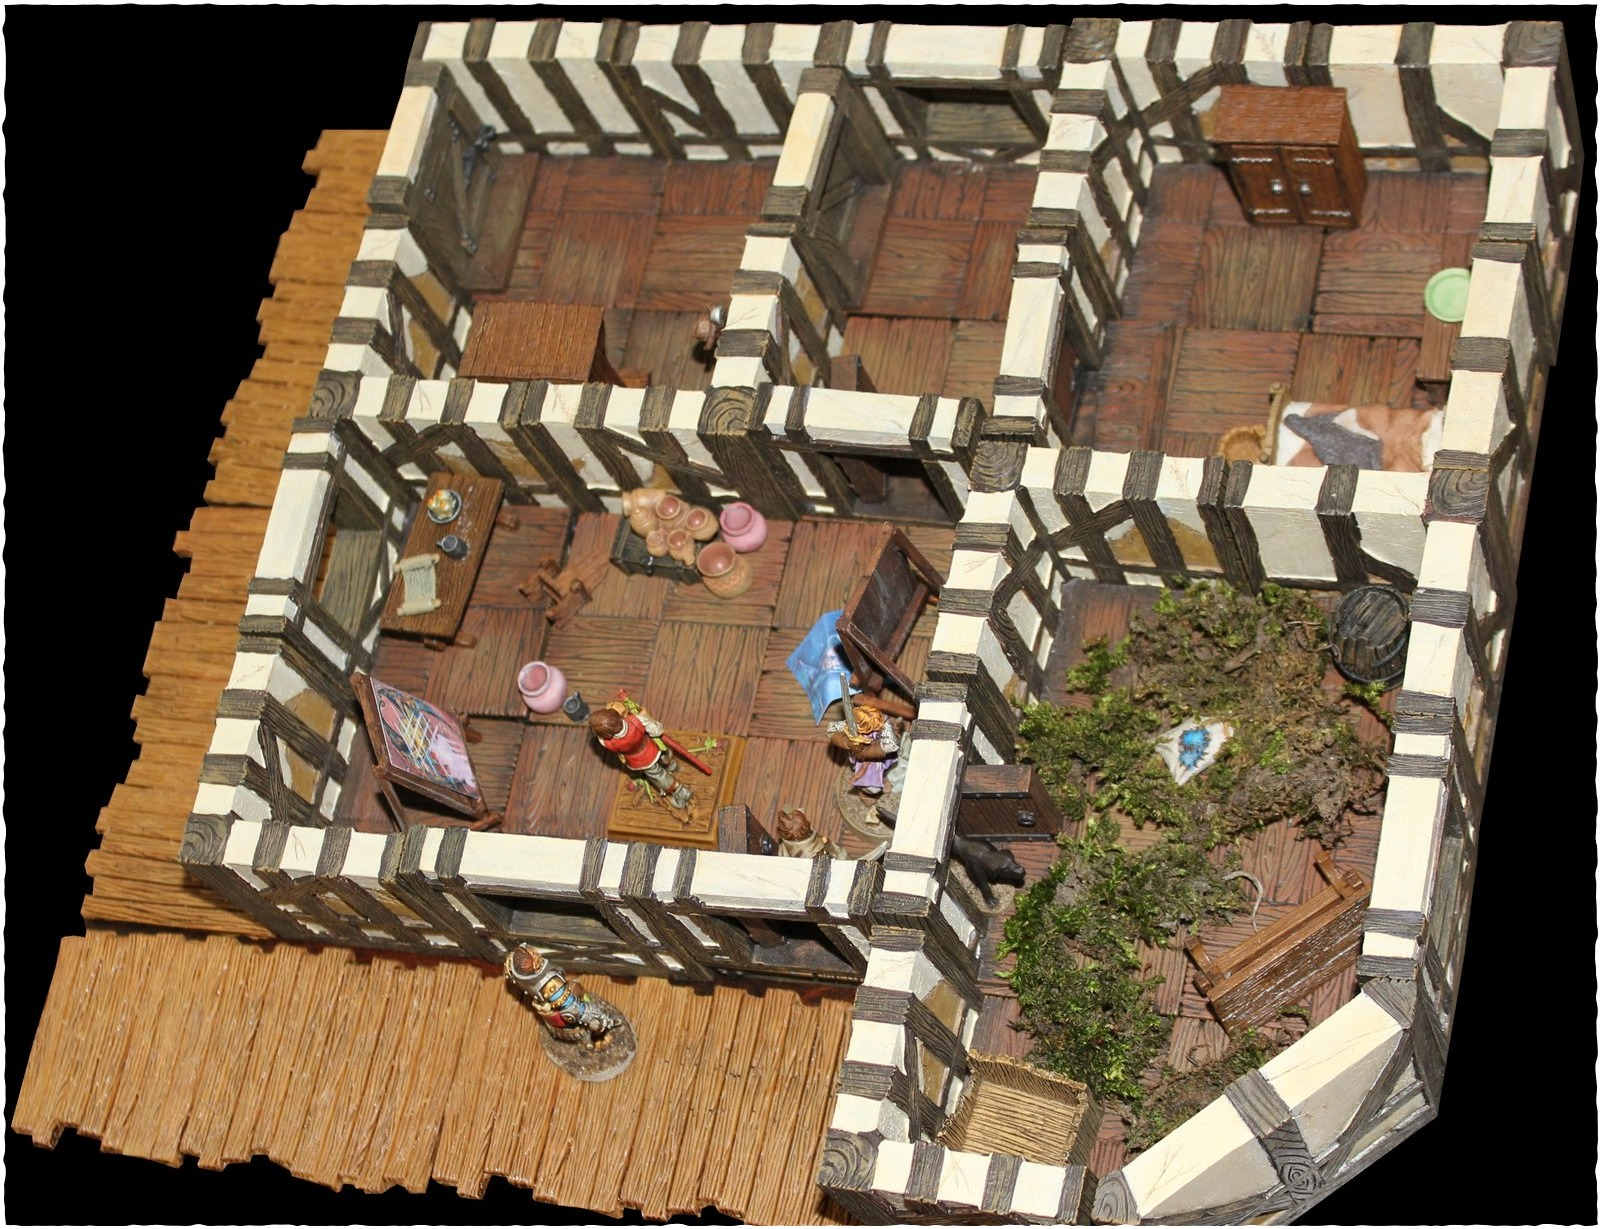
\includegraphics[width=0.4\textwidth]{images/Where-is-Salvator-Scream-562539967_mod.jpg}
	\caption{Where is Salvator Scream?}
	\label{fig:Where-is-Salvator-Scream-562539967}
\end{figure}

Salvator's studio stinks of must and mildew. At one time this room was a sanctuary where an inspired madman committed the visions of violence and horror in his head to canvas, but Salvator's latest work shows none of that brilliance.\hyperref[fig:Salvator-Scream-studio-562540993]{ Frustration must have taken hold of the artist, as he destroyed his own lackluster creations. }  \\

\begin{figure}[h]
	\centering
	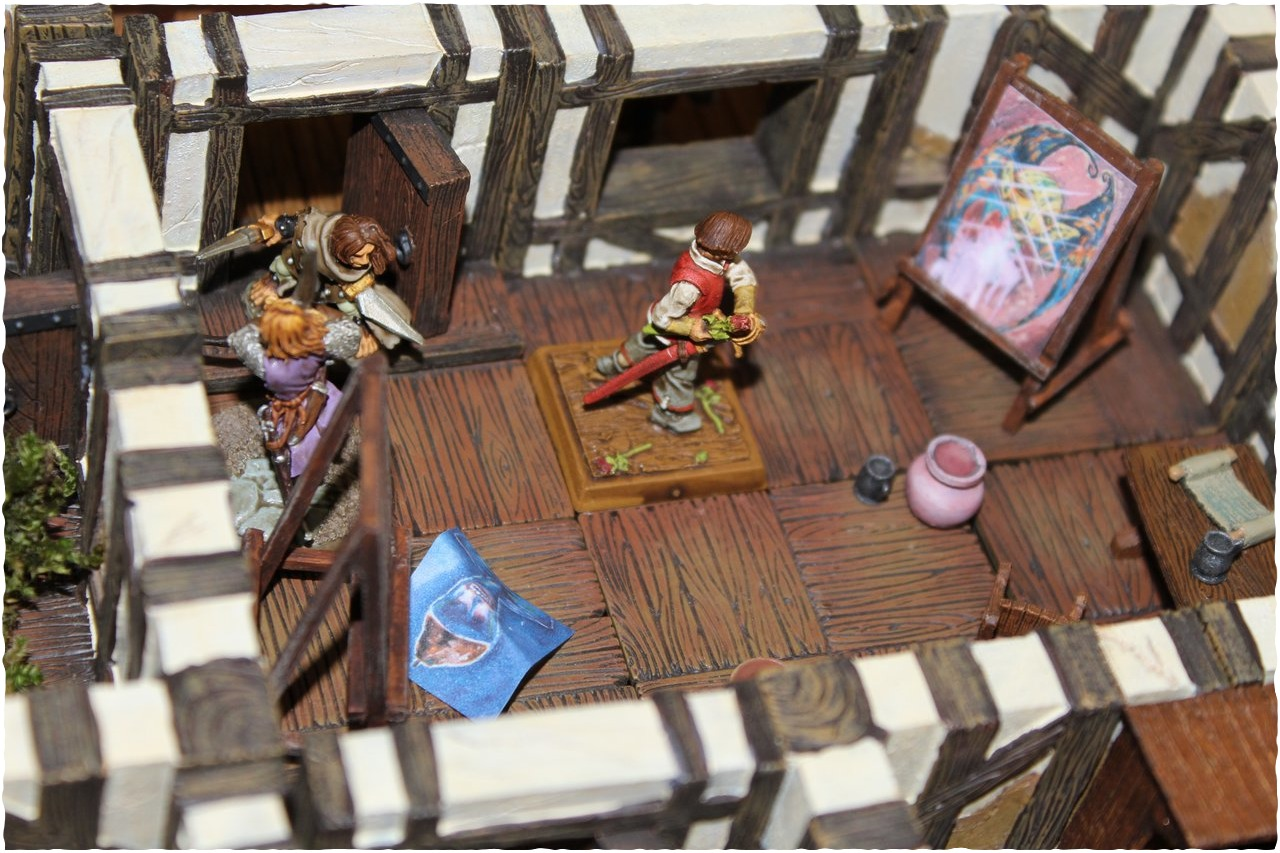
\includegraphics[width=0.4\textwidth]{images/Salvator-Scream-studio-562540993_mod.jpg}
	\caption{Salvator Scream studio}
	\label{fig:Salvator-Scream-studio-562540993}
\end{figure}

Outside the party comes across some of the emperor's men. Quint inquires about Salvator Scream's whereabouts and easily tricks the goons into admitting that mister Scream is a 'guest' at their master's. Seeing this as an easy opportunity to make some money, Corl, one of the thugs, offers to procure an audience with the emperor in exchange for a pay-off. He wants 25 gold sails, but is haggled down to a mere 5 gold pieces before he takes to companions to the emperor's poor excuse of a palace.\\

Emperor Pilts Swastel heartily welcomes the heroes back to his place and after graciously accepting their gift of a magic cloak as a tribute, he agrees to let them speak to the painter for a couple of minutes. He takes the companions into\hyperref[fig:Pilts-Swastel-emperor-of-Old-Korvosa-562541723]{ the building behind his throne } and leads them to a dark, unpleasant room, scarcely more than a cell, in which Salvator Scream is pining away. Pilts has no intention of leaving the party alone with the painter and sits down in a chair as he invites his guests to have their little conversation. The emperor feels comfortalbe in the company of his four personal bodyguards, who easily kicked the heroes' butts last time. \\

\begin{figure}[h]
	\centering
	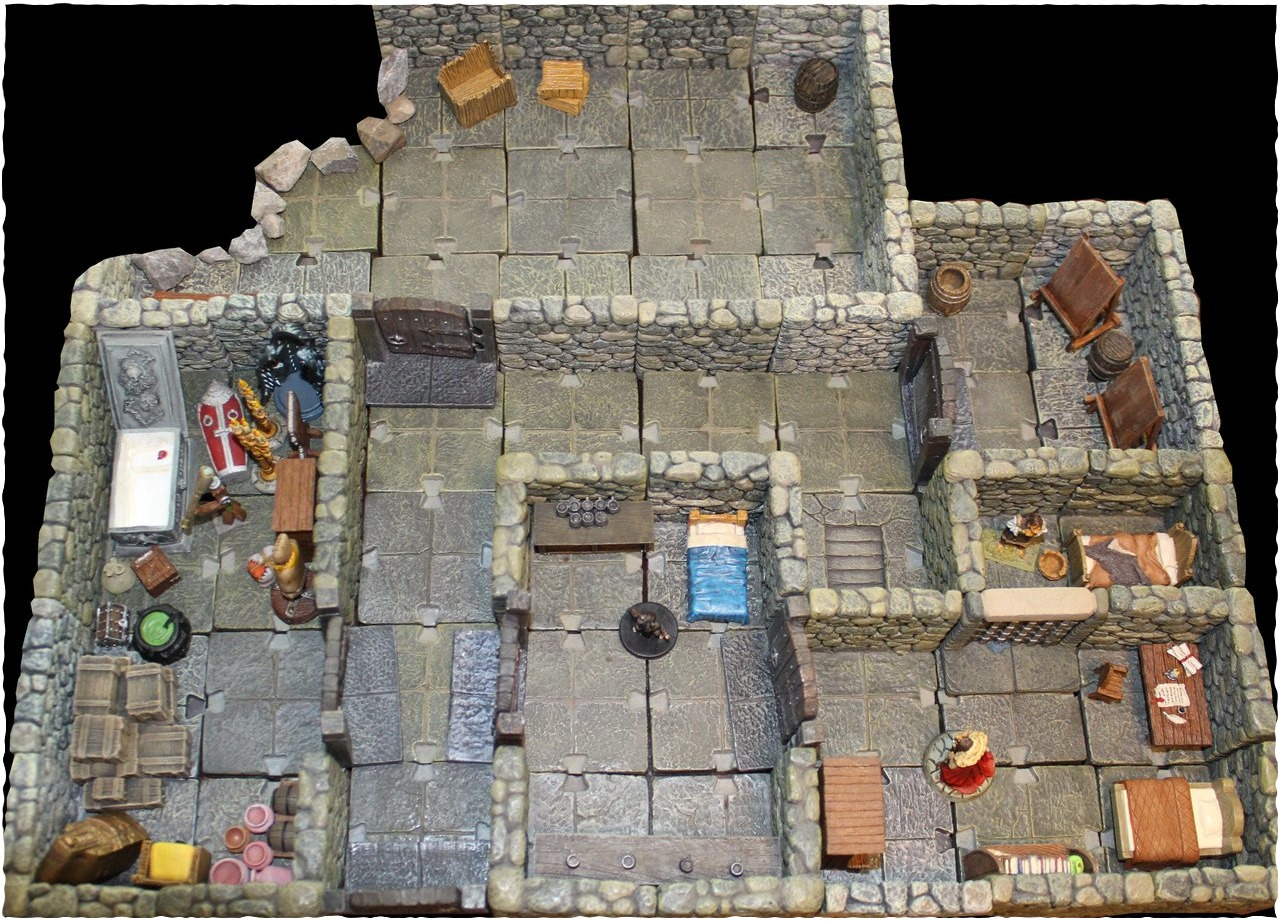
\includegraphics[width=0.4\textwidth]{images/Pilts-Swastel-emperor-of-Old-Korvosa-562541723_mod.jpg}
	\caption{Pilts Swastel, emperor of Old Korvosa}
	\label{fig:Pilts-Swastel-emperor-of-Old-Korvosa-562541723}
\end{figure}

Scream looks in bad shape and seems ill at ease with the emperor staring down his face. Still, the companions convince him to talk. His tale starts with Neolandus Kalepopolis, the seneschal of Castle Korvosa. The two of them became friends a few years ago and regularly shared drinks to discuss art, religion and history. Then, three months ago, things started going horribly wrong. First Scream lost his muze and and three weeks later Neolandus Kalepopolis showed up on his doorstep, on the morning of King Eodred's death. The seneschal was grievously wounded and had lethal poison running through his veins. Kalepopolis drifted between life and death for many weeks, but somehow the good man survived, taking even longer to fully recover. When he finally felt better, Neolandus entrusted Salvator Scream with the terrible truth of what had happened to him. He had discovered that Queen Ileosa was responsible for killing her husband and that she had enlisted the aid of the Red Mantis, a secret organisation of deadly assassins. Two of those dreaded killers in their red insectoid armor had tried to slay him, but Neolandus escaped, barely alive, fleeing to Old Korvosa.\\

Neolandus admitted that he had never been a fan of Ileosa, but in the final weeks of Eodred's life, she had somehow changed for the worse, whatever that entailed. The seneschal did not share more on this topic with Scream, claiming "the less the painter knew, the safer he'd be". Neolandus also realized that he the painter's humble shack was no safe place to hide any longer, so now that he finally felt better, he wanted to find another refuge. Scream suggested the Arkona's, Old Korvosa's only remaining noble family. Since the island had already been cut off from the mainland at this point, the Arkona's seemed like the safest place to stay. The seneschal had his doubts, but Scream convinced him there was no alternative. Moreover, the artist liked Glorio Arkona, to whom he had sold several of his paintings in the past. He took Neolandus Kalepopolis there and hasn't heard from him since. The Arkona's seemed nice enough when he delivered the seneschal to them and Salvator Scream had felt like he could trust the nobles.\\

That changed after Scream talked to Vencarlo Orisini. The fencing master never tried to hide his disdain for House Arkona and seemed convinced that the family was involved in all kinds of dark, criminal activities. He was so outspoken about his distrust for these nobles that it took Scream three visits, spread out over more than a week, to gather the courage to tell him that he had delivered Neolandus Kalepopolis into their hands. Orisini got raving mad when he heard that, claiming that the seneschal would have been better off in Ileosa's dungeons.\\

When the heroes inform Salvator Scream that Vencarlo was attacked by the Red Mantis and has disappeared after escaping the assassins, the painter gets even more worried. He has no idea where the fencing master could be, but if he's still on the island, he might very well have gone to the Arkona Palace to find the seneschal.\\

At this point Pilts Swastel interrupts the conversation. The content smile on his face shows that he is pleased with what he has just overheard, but now he claims that time is up - the cloak the heroes gave him only bought them so much time. Sjo shoots a glance of understanding at Quint and the bards spurts into action, suddenly casting a {\itshape haste} spell. Balian takes advantage of his accelerated actions to chop down one of the emperor's bodyguards with three heavy blows. Puk throws himself at Pilts Swastel and almost takes the man out with three vicious lashes. Spyder finishes the job by grabbing the surprised emperor by the throat and choking the life out of him. The remaining bodyguards back down when Sjo steps in front of them, growling like a mad dog. The fight ends as quickly as it began, just like the first confrontation with the emperor, only this time the companions are on the winning side. The emperor's rule is over! Sjo drags his dead body outside and throws it on the guillotine. Most of the emperor's men have already cleared the scene; some of them are glancing at the adventurers from a safe distance and witness how their precious leader loses his head under his own  {\itshape tall knife} . Sjo shouts out a challenge to them: "The emperor is dead! If I ever catch as much as the smell of you cowards, you'll suffer the same fate! Now RUN!" At that the mob disappears, leaving only a stupefied one-eyed gnome on the open-air balcony. When Sjo leans over him, the mute creature starts gesturing that he is innocent, pointing at the emperor's remains as the source of all evil. With a nod Sjo lets him go and the gnome jumps at the chance to get away. Quint comes out with his hand on Scream's shoulder. "You're free to go, Salvator, Swastel won't bother you again."\\

"So, what do we know about this Arkona dude?" Balian inquires. "We met him once, at the great council in the castle ...  He seemed pretty level-headed to me. And didn't we see his sister at the celebration in the Jeggare Museum, before the opera?"\\

"Yes, we did", Quint confirms. "I've picked up many rumors over the years. They say that the Arkona's are one of the richest families in Korvosa - if not the richest. Their home is supposed to be a magnificent marble castle, up on Garrison Hill. They do business with the distant nation of Vudra ... very lucrative, since they are one of the few trading companies allowed to import and export goods there. Most of their vessels never even make it to Korvosa, preferring to sell their cargo in the Inner Sea region instead.\\

The guards at their palace are Vudran too, as is Glorio's other half. Most people think he has a wife and two kids in Cheliax, but I've heard his spouse is a Vudran beauty who has never left her home country. She's raising his son and daughter there as well.\\

It was actually one of Glorio's forefathers who established the profitable relations with Vudra, a man named Nerio Arkona. He saved his house by pouring his last coins in a trading vessel, the {\itshape Reprieve} it was called ... hmm, must have been two and a half centuries ago, I reckon. Anyway, his journey was fraught with peril, but he survived and turned his enterprise into a smashing success. Upon his return, three years after he had left, he ordered the Arkona Palace built. Yes, he really managed to turn his fortune around, going from nearly bankrupt to filthy rich." "Still, why does Vencarlo think he is so dangerous?" Puk wonders. "Aren't the Arkona's known for their generosity, providing cheap housing for the poor and sometimes even handing out money in the streets?"\\

"They are", Quint nods. "The man is quite popular and respected in this district. But this image of the big-hearted benefactor hides a less admirable truth. I'm afraid Vencarlo may be right. I've also heard that the Arkona's are heavily involved in crime, through the Cerulean Society, to be exact. Korvosa's thieves' guild does some dirty business, but by never crossing the line and by paying a hefty vice tax, they can get away with it ... even with being a 'guild' in a city that allows none. What's their leader's name again? Boule! A brute of a man, if rumors be true."\\

"Doesn't really matter how good or bad our man is, I suppose", Sjo interjects. "We'll find out soon enough as I suggest we pay him a visit. What do you say?"\\

"I guess we must", Balian smiles. "Let's knock on his door for a cup of tea."\\

"Coffee", Quint remarks. "Vudrans drink a bitter black tea they call coffee."\\

